\documentclass{article}

\usepackage[utf8]{inputenc}
\usepackage[spanish]{babel}
\usepackage{graphicx}
\usepackage{amsmath}

\title{Modelos matemáticos discretos}
\author{Sua}
\begin{document}
\maketitle
\section{Ecuaciones en diferencias}
\subsection{Primer orden}

Tenemos 1000 pesos que vamos a invertir a un interés de 1\% mensual.

El valor de la inversión cuando han transcurrido $n$ meses es $$x_n=1000(1.01)^n$$
Una gráfica del resultado es:

\begin{center}
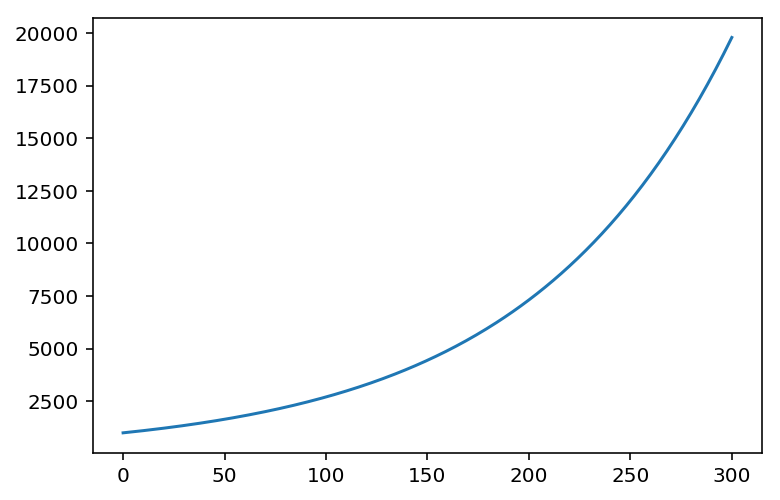
\includegraphics[width=4cm]{grafica}
\end{center}

Para encontrar este resultado, ocupamos que: $$\sum_{i=0}^{n-1}a^i=\frac{1-a^n}{1-a}$$

Algunos valores de la inversión:
\begin{center}
\begin{tabular}{|c|r|}
\hline
Mes & Valor \\
\hline
0 & 1000 \\
1 & 1010 \\
2 & 1021.1 \\
3 & 1030.301 \\
\hline
\end{tabular}
\end{center}

\subsection{Segundo orden}


\begin{center}
\huge
\textbf{YA ME SALIÓ}
\end{center}

Calcular los valores propios de $$A=
\begin{pmatrix}
1 & 2 \\
\pi & 4
\end{pmatrix}.
$$

\end{document}
